
\documentclass[a4paper]{report}

\usepackage[ngerman]{babel}
\usepackage[utf8]{inputenc}
\usepackage{longtable}
\usepackage{graphicx}
\usepackage{graphics}
\usepackage[pdfborder={0 0 0}]{hyperref}
\usepackage{geometry}
\usepackage{float}
\usepackage{fancyhdr}
\usepackage{titling}
\usepackage{csquotes}
\usepackage{minted}
\usepackage{xcolor}
\usepackage{verbatimbox}
\usepackage{textcomp}

\newcommand{\subtitle}[1]{%
  \posttitle{%
    \par\end{center}
    \begin{center}\large#1\end{center}
    \vskip0.5em}%
}

\newenvironment{fullgrayverb}
{\verbbox}
{\endverbbox\par\colorbox{lightgray}{\parbox{\textwidth}{\theverbbox}}\par}

\title{Netzwerk- und System-Management-Projekt}
\subtitle{Netzwerk- und Service-Struktur einer Fakultät}
\date{\today}
\author{Tom Wegener, 18INM/TZ}
\pretitle{%
  \begin{center}
  \LARGE
  
\includegraphics[width=6cm]{pictures/htwk-logo.jpg}\\[\bigskipamount]
}
\posttitle{\end{center}}

\geometry{a4paper, left=30mm, right=20mm,top=25mm,bottom=25mm}
  \fancyhead{}
  \fancyhead[L]{Tom Wegener, 18INM/TZ}
  \fancyhead[R]{Abschlussbericht NSM}
  \fancyfoot{}
  \fancyfoot[R]{\thepage}

\setlength{\parindent}{0em}


\begin{document}

\pagestyle{empty}

\maketitle
%
\includegraphics[width=5cm]{pictures/htwk-logo.jpg}

\newpage

\tableofcontents

\newpage

\pagestyle{fancy}

\setcounter{page}{1}

\chapter{Einleitung}

Für das Modul Netzwerk- und System-Management (NSM) sollen die Studierenden des Studiengangs "Informatik Master" der HTWK Leipzig die Infrastruktur einer Fakultät erstellen, die sich außerhalb des Universitäts-netzes befindet.

Das Projekt soll mit Hilfe von Netkit als virtuelle Infrastruktur realisiert werden und anschließend über Ansible konfiguriert werden. Zuletzt soll ein Bericht zu dem Netzwerk und der Umsetzung verfasst werden.

\section{Umgebung}

Das Projekt wurde nicht innerhalb der VM umgesetzt, sondern für bessere Performance direkt auf einem privaten Rechner. Auf dem Rechner ist eine Linux-Distribution, die auf Ubuntu 18.10 basiert, installiert. Dabei hat Ansible die Version 2.7.8 und nutzt die Python-Version 3.6.7. Anstatt der originalen Netkit-Version wurde \href{https://netkit-ng.github.io/}{Netkit-ng} genutzt, welches ein neueres Filesystem nutzt, das auf Debian wheezy basiert. Das war notwendig, um die notwendige Version von Python zur Verfügung zu haben, da Ansible mindestens Python der Version 2.7 benötigt.

Die Verbindung zwischen dem Host bzw. Ansible und den Netkit-VMs wird über SSH realisiert in einer Agent-less Architektur.

Durch die trotzdem veraltete Version des Netkit-File-Systems können einige Sachen nicht wie im Konzept beschrieben umgesetzt werden. Durch ein Update des File-Systems auf eine neuere Debian-Version, kann dies ermöglicht werden. Für dieses Projekt wurde versucht, die bereits vorhandene Software so wenig wie möglich zu verändern. Dementsprechend sind auch nur relevante Applikationen auf den VMs aktuell, es wurde kein generelles Update ausgeführt.

\chapter{Konzept}

Für das Netzwerk-Konzept wurde eine Struktur mit mehreren getrennten Subnetzen gewählt, das eine einfache Administration gewährleistet, eine Erweiterung erleichtert und es erleichtert sicherheits-relevante Änderungen schnell umzusetzen. Im Kapitel Netzwerke und Sub-Netzwerke wird auf die Struktur eingegangen, während im Kapitel Werkzeuge die benötigte Software kurz vorgestellt wird und im Kapitel FCAPS die Nutzung genauer erläutert wird.

\section{Netzwerke und Sub-Netzwerke}
Die Infrastruktur besteht grundlegend aus drei Subnetzen, sowie einem großen Netzwerk. Die Verbindung der Subnetze wird über das Kern-Netzwerk bzw. den Kern-Router ermöglicht. Zusätzlich zu dem Kern-Router hat jedes Subnetzwerk einen Router und der Anschluss über die Dark-Fiber-Leitung wird auch über einen Router realisiert. Die drei Subnetzwerke sind die demilitarisierte Zone (DMZ), das Server-Netzwerk und das Client-Netzwerk.
Verbunden wird alles über das Kern-Netzwerk, welches für sich auch ein eigenes Subnetz darstellt. Über dieses Netzwerk werden die verschiedenen Netzwerke verbunden. Die gesamte Infrastruktur ist vereinfacht in der Abbildung \ref{fig:model} grafisch dargestellt.

\begin{figure}
  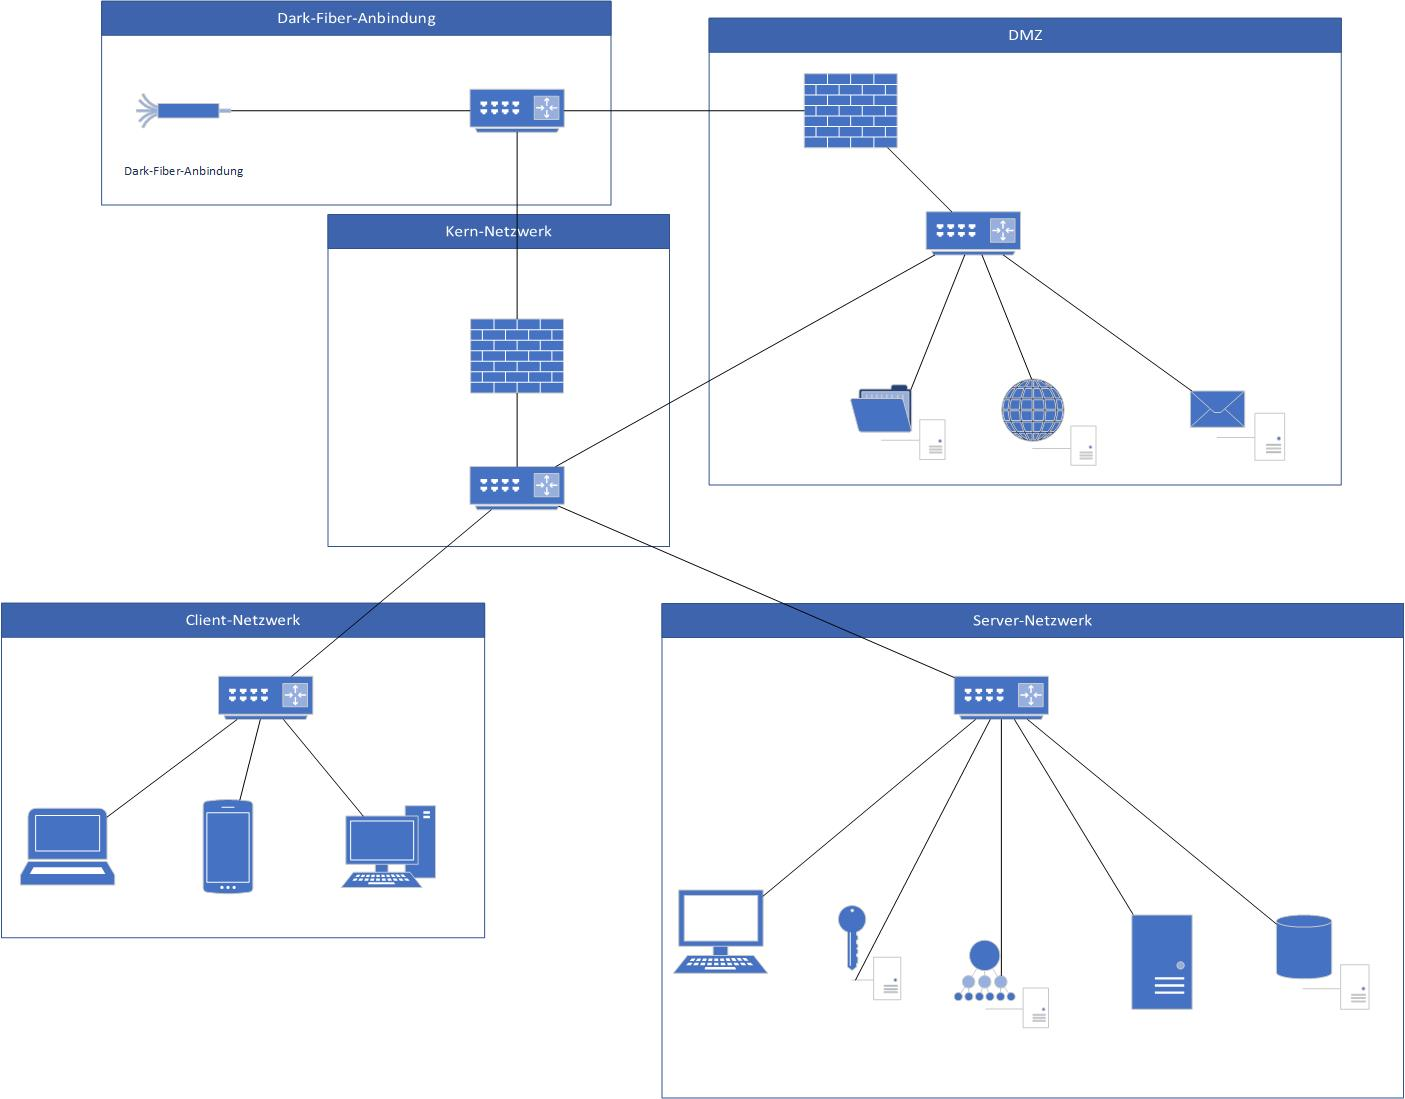
\includegraphics[width=\linewidth]{pictures/netzwerk-diagramm.jpg}
  \caption{Modell der Infrastruktur}
  \label{fig:model}
\end{figure}

In der Abbildung ist pro Netzwerk nur ein Router eingezeichnet, um die Übersichtlichkeit zu verbessern. Es sollte bei einer Umsetzung bedacht werden, dass es mindestens zwei gibt, um einerseits einen Ersatz bei einem Ausfall zu haben, aber auch, um  ein Load-Balancing zu ermöglichen.

\subsection{Das Kern-Netzwerk}
Das Kern-Netzwerk enthält die Router, die dafür zuständig sind, den Traffic der gesamten Infrastruktur abzuwickeln. Ausgenommen davon sind Zugriffe auf die Server der DMZ, die aus dem Internet heraus bzw. über die Dark-Fiber-Verbindung getätigt werden.

Die Routen werden statisch festgelegt und die Router wissen von den einzelnen Subnetzwerken und können dementsprechend den Traffic unterscheiden. Die Router der einzelnen Subnetzwerke wissen nur von den Adressen in dem jeweiligen Sub-Netzwerk und können nur zwischen Traffic für das eigene Netzwerk und die restliche Infrastruktur unterscheiden.

\subsection{Die Demilitarisierte Zone}
Die DMZ stellt alle Dienste bereit, die über das Internet erreichbar sein sollen, also einen Web-Server, einen Mail-Server und einen AAA-Server. Jedoch werden kritische Daten nicht auf Servern in der DMZ gespeichert, sondern sind auf Servern in dem Server-Netzwerk gespeichert, die jedoch über Server aus der DMZ erreichbar sind.

In der DMZ ist ein FTP-Server, der Daten aus dem Server-Netzwerk abfragt, der Web-Server, der Mail-Server, der genau so, wie der FTP-Server die Daten auch von Servern des Server-Netzwerkes nachlädt und ein DNS-Server. Eine GitLab-Instanz kann ebenfalls hier positioniert werden.

Als IP-Adress-Bereich wurde 10.0.2.0/24 gewählt, die Server haben also eine Adresse zwischen 10.0.2.0 und 10.0.2.255, während die 10.0.2.01 für den Router benutzt wird. Die Server haben alle eine festgelegte IP-Adresse, die innerhalb der Server und bei dem Router festgeschrieben wird.


\subsection{Das Server-Netzwerk}
Das Server-Netzwerk ist für die Bereitstellung von Daten und Diensten innerhalb der Fakultät zuständig. Zur Sicherheit sollten keine Daten aus diesem Subnetz direkt den Dark-Fiber-Router passieren, sondern maximal über einen Server der DMZ abgefragt werden und dann weitergeleitet werden.

Das Netzwerk enthält den für den AAA-Services benötigten Server, die benötigten Datenbanken, die Icinga-Instanz, sowie den Foreman-Server. Außerdem können spezifische weitere Services, wie die GitLab-Datenbank, in dem Netz realisiert werden.

Die AAA-Services können zum Beispiel über das RADIUS-Protokoll realisiert werden, das auch mit einer Authentifizierung über PAM erweitert kann und kann deshalb einfach mit den Linux-Clients realisiert werden.

Die Datenbanken sind ebenfalls in diesem Netzwerk realisiert, sind aber nur über die Server zu erreichen. Von den Datenbanken werden regelmäßig Backups angefertigt, die einerseits als unabhängig vom Netzwerk gelagert werden.

Zusätzlich ist im Server-Netzwerk ein Administrations-Rechner, der zur Verfügung steht, sollte die Verbindung zu dem Netzwerk über das Kern-Netzwerk abbrechen.

Als IP-Adress-Bereich wurde 10.0.3.0/24 gewählt, die Server haben dementsprechend eine Adresse zwischen 10.0.3.0 und 10.0.3.255, während die 10.0.3.01, ähnlich wie in der DMZ, für den Router benutzt wird. Die Server und Datenbanken haben alle eine festgelegte IP-Adresse, die innerhalb der Server und bei dem Router festgeschrieben wird.

\subsection{Das Client-Netzwerk}
Die Rechner der Angestellten der Fakultät, sowie der Studierenden der Fakultät, sind alle über das Client-Netzwerk verbunden. Die Administration erfolgt ebenfalls über einen Rechner im Client-Netz oder über den Administrations-Rechner im Server-Netzwerk.

Auf den Computern des Client-Netzwerkes ist das Betriebssystem Ubuntu-Linux installiert, sollte jedoch aufgrund von benötigter Software ein anderes Betriebssystem benötigt werden, kann das auch realisiert werden. Dabei wird Ubuntu genutzt, da es eine einfache Benutzung ermöglicht, eine große Auswahl an Software bietet und außerdem stabil ist. Außerdem wird die Administration über die kommerzielle Software Landscape von Canonical erleichtert.

Bei diesem Subnetz wurde der IP-Adress-Bereich 10.0.4.0/24 genutzt, die Adressen variieren dementsprechend zwischen 10.0.4.0 und 10.0.4.255, während auch hier der Router die Adresse 10.0.4.01 hat. Während die von der Fakultät gestellten Computer eine feste IP-Adresse haben, werden den zusätzlichen Geräten, die z.B. über eduroam verbunden werden, eine zufällige IP-Adresse zugewiesen, da eine feste Zuweisung auf Grund der Masse der möglichen Geräte, nicht realisierbar ist.

\section{Werkzeuge}
Generell soll das Netzwerk durch das Tool \href{www.theforeman.org}{Foreman} administriert werden. Foreman ermöglicht die Administration von Hosts und kann auch für die Administration von großen Netzwerken samt Routern, Clients und Servern genutzt werden. Über eine Web-Oberfläche wird es ermöglicht einen Überblick zu behalten, sowie die Provisionierung und die Konfiguration abzuwickeln.
Das Administrationstool wickelt die Konfiguration eigentlich über Puppet ab, kann jedoch durch Plugins erweitert werden, wie dem Ansible-Plugin. 

Ansible soll anstatt des in Foreman integrierten Puppet für die Konfiguration der Server genutzt werden. Die Konfigurationen der einzelnen Komponenten werden als playbooks angelegt und abgespeichert.

Sollte die Software kein anderes Betriebssystem als Ubuntu-Server benötigen kann zusätzlich das kommerzielle Management-Tool Landscape von Canonical benutzt werden. Es ermöglicht eine einfache Administration verschiedener Instanzen und kann die Auslastung, Zustand der Hardware und den Sicherheitszustand anzeigen. Landscape basiert aus einer Agent-Architektur, erfordern also einen Client auf den zu verwaltenden Rechnern.

Außerdem können Foreman und Landscape auch bei der Realisierung von FCAPS helfen.

\newpage

\section{FCAPS}
FCAPS ist ein Modell für das Management von Netzwerken bzw. Infrastrukturen, es ist ein Akronym für Fault-Management, Configuration-Management, Administration and Accounting Management, Performance Management und Security Management. FCAPS wird in diesem Fall über verschiedene Tools und mit Hilfe von Foreman realisiert.

Es wurde sich bewusst für FCAPS entschieden und nicht für FAB oder ITIL, da FCAPS sehr ausführlich die wichtigsten Bestandteile der Netzwerk-Management behandelt.


\subsection{Fault-Management}
Fault-Management bedeutet das frühzeitige Erkennen und Beheben von Fehlern innerhalb des Netzwerkes, das kann durch z.B. eine Icinga-Instanz realisiert werden. Alternativ kann auch ein anderes Werkzeug, wie z.B. Foreman, genutzt werden, welches mehrere Teile von FCAPS in sich vereinigt.

Foreman überprüft die Anwesenheit und Funktionalität von Hosts durch puppet-nodes, außerdem kann durch ein Plugin zentralisiertes Logging umgesetzt werden. Sollte ein Fehler auftreten, der unter eine bestimmte Einstufung, wie z.B. ''kritisch'' fällt, kann eine Benachrichtigung gesendet werden, außerdem wird auch ein vereinfachtes Handeln unterstützt, solange eine Verbindung zum Host besteht, können Logs abgerufen werden, Konfigurationen erneut angewendet werden oder Updates gefahren werden.

Für ein übersichtliches Logging müssen die Logs in verschiedene Stufen eingeteilt werden. Es empfiehlt sich, diese einerseits nach Gefahr für die weitere Funktionalität einzuteilen, wie auch in die verschiedene Komponenten. So können Logs, wie z.B. ''critical: infrastructure: lost connection to mail-server'' schnell verstanden werden.

\subsection{Configuration Management}
Das Konfigurationsmanagement wird über Ansible abgewickelt. Dabei werden die einzelnen benötigten Dienste als Konfigurationen in playbooks angelegt, die einen entsprechenden Namen haben, sollte ein Host ausfallen, kann in der host-Datei ein neuer Host der entsprechenden Gruppe hinzugefügt werden. Theoretisch können die Konfigurationen der Router ebenfalls über playbooks abgespeichert werden. 

Durch eine Integration von Ansible in Foreman über das dazugehörige Plugin kann die Ausführung von playbooks einfach umgesetzt werden, sowie die Ausführung überwacht werden. Die Ergebnisse der Ausführung werden bei Foreman je Host aufgelistet.

\subsection{Administration and Accounting Management}
''Administration and Accounting Management'' beinhaltet das Management der Accounts und der für die Abrechnung benötigten Nutzungsdaten. Das beinhaltet die AAA-Services, die z.B. über das RADIUS-Protokoll realisiert werden können. Die AAA-Services beinhalten Authentication, Authorization and Accounting. Damit ist einerseits eine Überprüfung der Identität des bzw. der Nutzenden möglich und dementsprechend auch eine Gewährung der Zugriffsrechte und andererseits eine Abrechnung der genutzten Dienste.

Für das Accounting-Management, sowie die Nutzenden-Verwaltung muss ein Konzept erstellt werden, wie die Verwaltung geschieht und wie die (Zugriffs-)Rechte realisiert und zugeteilt werden können. Grundlegend kann die Zuteilung über Gruppen realisiert werden, in die die Nutzenden je nach ihrem Aufgabengebiet eingeteilt werden. Zusätzliche Rechte können auch verteilt werden.

\subsection{Performance Management}
''Performance Management'' bedeutet die Überwachung der Performance aller Komponenten des Netzwerkes. Dabei muss die Auslastung der Server, die Gesundheit und das Alter von Festplatten und anderen (Netzwerk-)Komponenten überwacht werden.

Grundlegendes Performance-Monitoring kann über Landscape abgewickelt werden, aber auch die Icinga-Instanz kann eine Überwachung ermöglichen. 
Der Foreman-Server kann ähnliche Daten wie die Icinga-Instanz bereitstellen.

Das Performance-Management ermöglicht außerdem Hilfe bei den Teilen Fault Management und Security Management, da eine ungewöhnliche Auslastung verschiedener Bestandteile ein Indiz für ein Problem sein kann.

\newpage
\subsection{Security Management}
Security Management bedeutet sich über die Sicherheit der Infrastruktur bewusst zu sein und diese so gut wie möglich zu verbessern. Das beinhaltet die physische, sowie die digitale Sicherheit.

Das Security Management dient dem Schutz der Daten und Programme innerhalb des Netzwerkes.

Die physische Sicherheit kann grundlegend durch eine Zugangskontrolle zu den Räumen in denen die Server stehen erreicht. Jedoch werden noch weitere Schritte benötigt.

Die digitale Sicherheit kann unter Anderem durch IPSec realisiert werden, außerdem muss ein Überblick über wichtige Sicherheits-Updates beibehalten werden und diese durch das Konfigurations-Management aufgespielt werden.

Die Authorisierung für die Dienste und das Netzwerk wird über den AAA-Server realisiert. Dabei wird strengstens darauf geachtet, dass die einzelnen Gruppen möglichst wenig Rechte haben, das erfordert zwar einen erhöhten Administrationsaufwand, verbessert aber auch die Sicherheit des Netzwerkes.

Ein weitere Möglichkeit das Netzwerk zu sichern ist die Verschlüsselung des gesamten Traffics. So ist es wichtig, TLS auch innerhalb des Netzwerkes zu nutzen.

Außerdem wird der Zugriff auf z.B. das Server-Netzwerk aus dem Internet eingeschränkt. Es soll nur möglich sein aus dem Client-Netzwerk und der DMZ auf Daten, die auf diesen Servern liegen, zugegriffen werden. Außerdem werden über die beiden Firewalls die Zugriffe zusätzlich beschränkt und verschiedenen IP-Adressen geblockt.

Über Landscape kann überwacht werden, welche Sicherheits-Updates die Software, die auf den Rechnern installiert ist, noch ausstehend sind.

Zusätzlich sollte eine einfache Möglichkeit bereitgestellt werden, die Administrierenden zu kontaktieren, wenn eine Sicherheitslücke gefunden wird.
\chapter{Umsetzung}

Für die Umsetzung musste statt dem originalen Netkit Netkit-ng genutzt werden, welches python2.7 unterstützt, das für Ansible benötigt wird. Ein Update der Netkit-Instanzen auf python2.7 war auf Grund des Alters des File-Systems nicht möglich.

Es wurde eine wie in \ref{fig:model} Topologie erzeugt und über statische Routen, die in den .startup-Skripten festgelegt werden, eine grundlegende Netzwerk-Kommunikation ermöglicht. 
Die virtuellen Maschine, die mit ''r'' enden, sind die Router, die die Herzstücke des Netzwerkes bzw. der Subnetzwerke darstellen. 
Außerdem fangen die Namen der Maschinen mit dem Subnetzwerk an, zu dem sie gehören. 
So ist ''server-r'' der Router des Server-Netzwerkes, während ''server-foreman'' der Foreman-Server im Server-Netzwerk ist.

Die virtuellen Maschinen kriegen zusätzlich einen Arbeitsspeicher von 256 MB, um die Installation von Programmen zu ermöglichen.

Außerdem werden die einzelnen Netzwerk-Anschlüsse aufgelistet. Die TAP-Verbindung wird bei der ''darkfiber-r''-VM außerdem auch in der lab.conf festgelegt.

\section{Darkfiber}
Über die VM ''darkfiber-r'' wird eine Internet-Anbindung realisiert, wie sie in den Anforderungen gefordert wird. Die VM hat drei Anschlüsse, einer ist die Verbindung zu dem Internet bzw. die Dark-Fiber-Anbindung, die zweite Leitung führt zu dem Kern-Subnetzwerk, während die dritte Leitung zu der demilitarisierten Zone führt.

\section{Kern-Subnetz}
Über das Kern-Subnetz werden für alle Subnetze eine Verbindung zu jeweils anderen Subnetzen zur Verfügung gestellt, sowie auch die Verbindung zum Internet. Die Verbindung wird über statische Routen ermöglicht, die beim Startup angelegt werden.

\section{DMZ}
In der DMZ, also der demilitarisierten Zone, stehen die Server, die über das Internet erreichbar sein sollen. Dementsprechend ist der Web-Auftritt der Fakultät, sowie der Mail-Server und verschiedenen andere Dienste in der DMZ vertreten, sowie auch ein DNS-Server.

\section{Server-Subnetz}
In dem Server-Subnetz sind die verschiedenen Server der Fakultät enthalten, die für Datenspeicherung und Datenverarbeitung benötigt werden. Außerdem sind die Server, die für die Administration des Netzwerkes benötigt werden, wie die Icinga-Instanz und der Foreman-Server, ebenfalls in diesem Netzwerk vertreten. Auf sie kann über den Computer in dem Subnetz zugegriffen werden oder über Computer aus den anderen Subnetzen, jedoch nicht direkt über den Darkfiber-Router.

\section{Client-Subnetz}
Das Client-Subnetz ist mit dem Kern-Subnetz verbunden und kann über den Kern-Router eine Verbindung zu den anderen Subnetzen und zu dem Server aufbauen. Zu dem Client-Subnetz gehören einerseits alle fest verbauten Computer der Computer-Pools, sowie die Computer der Lehrenden und der weiteren Angestellten. Außerdem sind verschiedenen Wireless-Access-Points auch mit diesem Netzwerk verbunden, darüber können die Studierenden sich mit dem Internet verbinden.

\section{Ausblick}
Bei der Implementation war es nicht möglich alles zu realisieren. Einerseits liegt das an der Version des Netkit-File-Systems, welches nur Debian wheezy unterstützt und eine Erweiterung nicht im Bearbeitungszeitraum möglich war. Andererseits wurde kommerzielle Software im Konzept zur Nutzung vorgeschlagen, die nicht in der Realisierung genutzt werden konnte.

Außerdem war die ausführliche Nutzung von Foreman aufgrund der Virtualisierung nicht möglich.

Des Weiteren war es aufgrund der Größe des konzipierten Netzwerkes nicht möglich alle Dienste zu realisieren.
\chapter{Zusammenfassung}
Leider ist Netkit ein älteres Projekt, welches damit auch ältere Software als Basis verwendet. Besonders lässt sich das ältere File-System und der ältere Kernel betonen. Bei beiden ist die neueste offizielle Version von 2016, diese ist jedoch nicht stabil und voll funktionsfähig.

Eine andere Version, also Netkit-NG, hat ebenfalls eine veraltete Debian-Version und auch einen alten Kernel. Durch das erhöhte Alter ist die Kompatibilität zu einigen Programmen nicht gewährleistet.

Trotzdem kann die grundlegende Infrastruktur damit virtuell errichtet und ausprobiert werden.

Die Nutzung von Subnetzwerken verbessert die Sicherheit und vereinfacht die Organisation und Administration des Netzwerkes. Die Einteilung der benötigten Teile in die vier Schwerpunkte Clients, Server, DMZ und Internet- bzw. Dark-Fiber-Anbindung passt zu diesem Ansatz.

Die Verwendung von verschiedenen Programmen zur Verwaltung des Netzwerkes verkompliziert zwar das Management, da nicht alle Informationen innerhalb einer Oberfläche gesammelt und die Hosts mit Hilfe dieser kontrolliert werden können. Die erwähnte Software sind nur Vorschläge, wie das Netzwerk administriert werden kann, sie müssen mit genaueren Anforderungen evaluiert werden. Foreman bietet hier jedoch einen Lösungsansatz für das erste Problem, weil sich durch Plugins viel Funktionalität in dem Programm vereint oder sich vereinen lässt.


%\chapter{Anhang}
\section{Glossar}

\subsection{PXE}

\subsection{AAA-Services}
''Authentication, Authorization and Accounting''

\end{document}
